\documentclass[border=18pt,tikz]{standalone}
\usepackage{amsmath,amssymb,bm}
\usetikzlibrary{arrows.meta,positioning,calc,decorations.pathreplacing,fit,backgrounds}

% ============================================================
%  arch_common.tex  --  shared TikZ styles for MTP-PINN figures
%  All fonts bumped to \large; inner sep generous; no overlaps.
% ============================================================
\newcommand{\ArchBlockFont}{\large}
\newcommand{\ArchPhaseHdr}{\large\bfseries\color{black!80}}

%% --- Colour palette --------------------------------------------------------
\definecolor{KinFill}{RGB}{224,247,250}
\definecolor{KinDraw}{RGB}{0,131,143}
\definecolor{PhyFill}{RGB}{255,243,224}
\definecolor{PhyDraw}{RGB}{230,81,0}
\definecolor{NrmFill}{RGB}{243,229,245}
\definecolor{NrmDraw}{RGB}{106,27,154}
\definecolor{CatFill}{RGB}{255,249,196}
\definecolor{CatDraw}{RGB}{245,127,23}
\definecolor{MlpFill}{RGB}{227,242,253}
\definecolor{MlpDraw}{RGB}{21,101,192}
\definecolor{TanhFill}{RGB}{237,231,246}
\definecolor{TanhDraw}{RGB}{123,31,162}
\definecolor{AddFill}{RGB}{241,248,233}
\definecolor{AddDraw}{RGB}{85,139,47}
\definecolor{OutFill}{RGB}{232,245,233}
\definecolor{OutDraw}{RGB}{46,125,50}
\definecolor{LossFill}{RGB}{255,235,238}
\definecolor{LossDraw}{RGB}{183,28,28}
\definecolor{PhysBpFill}{RGB}{255,248,225}
\definecolor{PhysBpDraw}{RGB}{249,168,37}
\definecolor{NoteFill}{RGB}{245,245,245}
\definecolor{NoteDraw}{RGB}{100,100,100}

%% --- TikZ styles -----------------------------------------------------------
\tikzset{
  every node/.style={align=center},
  line cap=round,
  %% base block
  blk/.style={
    draw=gray!55,
    line width=1.6pt,
    rounded corners=6pt,
    inner sep=14pt,
  },
  %% domain blocks
  kinBlk/.style={
    blk, fill=KinFill, draw=KinDraw,
    minimum width=4.2cm,
    font=\ArchBlockFont,
  },
  phyBlk/.style={
    blk, fill=PhyFill, draw=PhyDraw,
    minimum width=5.8cm,
    font=\ArchBlockFont,
  },
  nrmBlk/.style={
    blk, fill=NrmFill, draw=NrmDraw,
    minimum width=4.0cm,
    font=\ArchBlockFont,
  },
  catBlk/.style={
    blk, fill=CatFill, draw=CatDraw,
    minimum width=2.2cm,
    font=\ArchBlockFont,
  },
  mlpBlk/.style={
    blk, fill=MlpFill, draw=MlpDraw,
    minimum width=3.6cm,
    font=\ArchBlockFont,
  },
  fcBlk/.style={
    blk, fill=MlpFill, draw=MlpDraw,
    minimum width=3.4cm,
    font=\ArchBlockFont,
  },
  tanhBlk/.style={
    blk, fill=TanhFill, draw=TanhDraw,
    minimum width=3.4cm,
    font=\ArchBlockFont,
  },
  outBlk/.style={
    blk, fill=OutFill, draw=OutDraw,
    minimum width=3.4cm,
    font=\ArchBlockFont,
  },
  addBlk/.style={
    circle,
    draw=AddDraw,
    fill=AddFill,
    line width=1.5pt,
    minimum size=1.4cm,
    font=\LARGE\bfseries,
  },
  gtBlk/.style={
    blk, draw=NoteDraw, fill=NoteFill,
    line width=1.2pt,
    rounded corners=5pt,
    inner sep=12pt,
    font=\ArchBlockFont,
    minimum width=3.2cm,
  },
  lossBlk/.style={
    blk, fill=LossFill, draw=LossDraw,
    line width=1.4pt,
    inner sep=16pt,
    font=\ArchBlockFont,
  },
  bpBlk/.style={
    blk, fill=PhysBpFill, draw=PhysBpDraw,
    inner sep=10pt,
    font=\ArchBlockFont,
  },
  %% arrows
  arr/.style={
    -{Stealth[length=11pt,width=9pt]},
    line width=1.8pt,
    black!80,
  },
  darr/.style={
    -{Stealth[length=9pt,width=7.5pt]},
    line width=1.5pt,
    dashed,
    dash pattern=on 5pt off 3pt,
    black!50,
  },
  bparr/.style={
    -{Stealth[length=11pt,width=9pt]},
    line width=1.8pt,
    PhyDraw!90,
    rounded corners=4pt,
  },
  %% edge labels
  dim/.style={
    font=\large,
    fill=white,
    inner sep=3pt,
    above=1pt,
    midway,
    sloped=false,
  },
  diml/.style={
    font=\large,
    fill=white,
    inner sep=3pt,
    below=1pt,
    midway,
  },
  phaseHdr/.style={
    font=\ArchPhaseHdr,
    inner sep=0pt,
    outer sep=0pt,
    anchor=south west,
  },
}


\def\BH{4.6cm}

\begin{document}
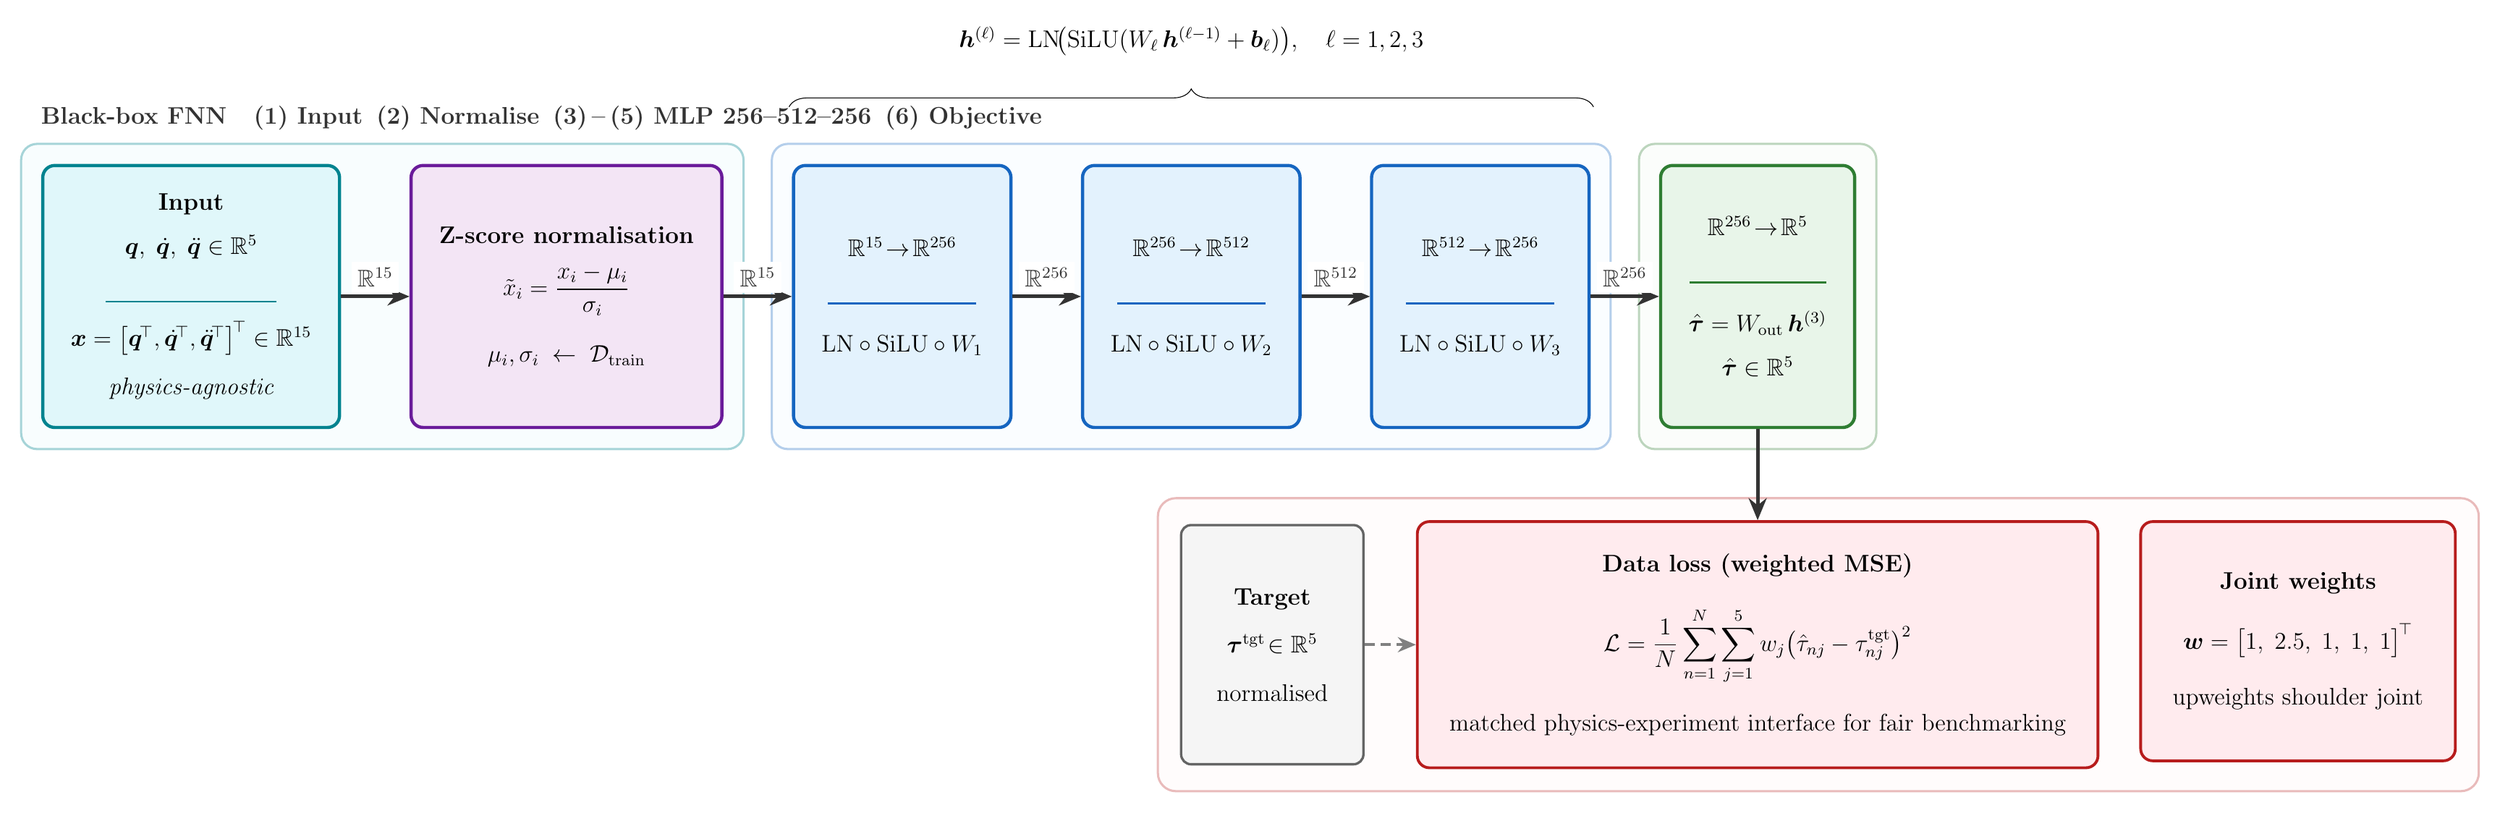
\begin{tikzpicture}[node distance=1.2cm]

%%═══════════════════════════════ INPUT ═══════════════════════════════════════

\node[kinBlk, minimum height=\BH, minimum width=4.2cm] (IN) {%
  \textbf{Input}\\[8pt]
  $\bm{q},\;\dot{\bm{q}},\;\ddot{\bm{q}}\in\mathbb{R}^{5}$\\[10pt]
  \textcolor{KinDraw}{\rule{3.0cm}{0.9pt}}\\[8pt]
  $\bm{x}=\bigl[\bm{q}^{\!\top},\dot{\bm{q}}^{\!\top},\ddot{\bm{q}}^{\!\top}\bigr]^{\!\top}
    \in\mathbb{R}^{15}$\\[10pt]
  {\large\itshape physics-agnostic}
};

\node[nrmBlk, minimum height=\BH, minimum width=4.0cm, right=1.2cm of IN] (NORM) {%
  \textbf{Z-score normalisation}\\[10pt]
  $\displaystyle\tilde{x}_{i}=\frac{x_{i}-\mu_{i}}{\sigma_{i}}$\\[14pt]
  $\mu_{i},\sigma_{i}\;\leftarrow\;\mathcal{D}_{\mathrm{train}}$
};

\node[mlpBlk, minimum height=\BH, minimum width=3.6cm, right=1.2cm of NORM] (H1) {%
  $\mathbb{R}^{15}\!\to\!\mathbb{R}^{256}$\\[10pt]
  \textcolor{MlpDraw}{\rule{2.6cm}{0.9pt}}\\[10pt]
  $\mathrm{LN}\circ\mathrm{SiLU}\circ W_{1}$
};

\node[mlpBlk, minimum height=\BH, minimum width=3.6cm, right=1.2cm of H1] (H2) {%
  $\mathbb{R}^{256}\!\to\!\mathbb{R}^{512}$\\[10pt]
  \textcolor{MlpDraw}{\rule{2.6cm}{0.9pt}}\\[10pt]
  $\mathrm{LN}\circ\mathrm{SiLU}\circ W_{2}$
};

\node[mlpBlk, minimum height=\BH, minimum width=3.6cm, right=1.2cm of H2] (H3) {%
  $\mathbb{R}^{512}\!\to\!\mathbb{R}^{256}$\\[10pt]
  \textcolor{MlpDraw}{\rule{2.6cm}{0.9pt}}\\[10pt]
  $\mathrm{LN}\circ\mathrm{SiLU}\circ W_{3}$
};

\node[outBlk, minimum height=\BH, minimum width=3.4cm, right=1.2cm of H3] (OUT) {%
  $\mathbb{R}^{256}\!\to\!\mathbb{R}^{5}$\\[10pt]
  \textcolor{OutDraw}{\rule{2.4cm}{0.9pt}}\\[10pt]
  $\hat{\bm{\tau}}=W_{\mathrm{out}}\,\bm{h}^{(3)}$\\[8pt]
  $\hat{\bm{\tau}}\in\mathbb{R}^{5}$
};

%% ── Forward-pass arrows ────────────────────────────────────────────────────
\draw[arr](IN)  --node[dim]{$\mathbb{R}^{15}$}  (NORM);
\draw[arr](NORM)--node[dim]{$\mathbb{R}^{15}$}  (H1);
\draw[arr](H1)  --node[dim]{$\mathbb{R}^{256}$} (H2);
\draw[arr](H2)  --node[dim]{$\mathbb{R}^{512}$} (H3);
\draw[arr](H3)  --node[dim]{$\mathbb{R}^{256}$} (OUT);

%% ── MLP brace annotation ───────────────────────────────────────────────────
\coordinate (BL) at ([yshift=1.0cm, xshift=-0.05cm]H1.north west);
\coordinate (BR) at ([yshift=1.0cm, xshift= 0.05cm]H3.north east);
\draw[decorate, decoration={brace,amplitude=9pt}]
  (BL)--(BR)
  node[midway,above=22pt,font=\large\itshape]{%
    $\bm{h}^{(\ell)}=\mathrm{LN}\!\bigl(\mathrm{SiLU}(W_\ell\,\bm{h}^{(\ell-1)}+\bm{b}_\ell)\bigr),\quad\ell=1,2,3$};

%% ── Background group fills ─────────────────────────────────────────────────
\begin{scope}[on background layer]
  \node[fit=(IN)(NORM), inner sep=10pt, draw=KinDraw!35, fill=KinFill!22,
        rounded corners=8pt, line width=1.1pt]{};
  \node[fit=(H1)(H2)(H3), inner sep=10pt, draw=MlpDraw!32, fill=MlpFill!18,
        rounded corners=8pt, line width=1.1pt]{};
  \node[fit=(OUT), inner sep=10pt, draw=OutDraw!32, fill=OutFill!18,
        rounded corners=8pt, line width=1.1pt]{};
\end{scope}

%% ═══════════════════════════════════════════════════════════════════════════
%%  ROW 2 : Loss block (directly below OUT, no gap)
%% ═══════════════════════════════════════════════════════════════════════════
\coordinate (LossTop) at ($(OUT.south)+(0,-1.6cm)$);

\node[lossBlk, anchor=north, minimum height=4.2cm, minimum width=11.0cm]
  (LOSSA) at (LossTop) {%
    \textbf{Data loss (weighted MSE)}\\[14pt]
    $\displaystyle
      \mathcal{L}
      =\frac{1}{N}\sum_{n=1}^{N}\sum_{j=1}^{5}
       w_{j}\bigl(\hat{\tau}_{nj}-\tau^{\mathrm{tgt}}_{nj}\bigr)^{2}$\\[14pt]
    {\large matched physics-experiment interface for fair benchmarking}
};

\node[lossBlk, anchor=north west, minimum height=4.2cm, minimum width=5.5cm]
  (LOSSB) at ($(LOSSA.north east)+(0.7,0)$) {%
    \textbf{Joint weights}\\[14pt]
    $\bm{w}=\bigl[1,\;2.5,\;1,\;1,\;1\bigr]^{\!\top}$\\[14pt]
    {\large upweights shoulder joint}
};

\node[gtBlk, anchor=east, minimum height=4.2cm]
  (GT) at ($(LOSSA.west)-(0.9,0)$) {%
    \textbf{Target}\\[10pt]
    $\bm{\tau}^{\mathrm{tgt}}\!\in\mathbb{R}^{5}$\\[10pt]
    {\large normalised}
};

%% ── Loss arrows ────────────────────────────────────────────────────────────
\draw[arr] (OUT.south) -- ++(0,-0.3) -| (LOSSA.north);
\draw[darr](GT.east)   -- (LOSSA.west);

%% ── Loss group fill ────────────────────────────────────────────────────────
\begin{scope}[on background layer]
  \node[fit=(GT)(LOSSA)(LOSSB), inner sep=11pt,
        draw=LossDraw!30, fill=LossFill!15,
        rounded corners=9pt, line width=1.1pt]{};
\end{scope}

%% ── Title header ───────────────────────────────────────────────────────────
\node[phaseHdr] at ($(IN.north west)+(0,0.6cm)$){%
  \textbf{Black-box FNN}\quad
  \textbf{(1)} Input\enspace
  \textbf{(2)} Normalise\enspace
  \textbf{(3)\,--\,(5)} MLP 256\textendash512\textendash256\enspace
  \textbf{(6)} Objective
};

\end{tikzpicture}
\end{document}


%% --- Forward pass -----------------------------------------------------------
\node[kinBlk, minimum height=\Bh, minimum width=3.08cm]
  (IN) {%
    \textbf{Rigid kinematics}\\[7pt]
    $\bm{q},\dot{\bm{q}},\ddot{\bm{q}}\in\mathbb{R}^5$\\[7pt]
    \textcolor{KinDraw}{\rule{2.1cm}{0.72pt}}\\[7pt]
    $\bm{x}=[\bm{q}^{\!\top},\dot{\bm{q}}^{\!\top},\ddot{\bm{q}}^{\!\top}]^{\!\top}\in\mathbb{R}^{15}$\\[10pt]
    {\footnotesize\itshape (no \(\bm{x}_{\mathrm{phy}}\);\;physics-agnostic baseline)}
  };

\node[nrmBlk, minimum height=\Bh, minimum width=3.08cm,
      right=of IN]
  (NORM) {%
    \textbf{Z-score}\\[9pt]
    $\tilde{x}_i=\dfrac{x_i-\mu_i}{\sigma_i}$\\[11pt]
    $\mu_i,\sigma_i\leftarrow \mathcal{D}_{\mathrm{train}}$
  };

\node[mlpBlk, minimum height=\Bh, minimum width=2.78cm, right=of NORM]
  (H1) {%
    $\mathbb{R}^{15}\rightarrow\mathbb{R}^{256}$\\[9pt]
    \textcolor{MlpDraw}{\rule{2.0cm}{0.72pt}}\\[9pt]
    $\mathrm{LN}\circ\sigma\circ W_{1}$
  };

\node[mlpBlk, minimum height=\Bh, minimum width=2.78cm, right=of H1]
  (H2) {%
    $\mathbb{R}^{256}\rightarrow\mathbb{R}^{512}$\\[9pt]
    \textcolor{MlpDraw}{\rule{2.0cm}{0.72pt}}\\[9pt]
    $\mathrm{LN}\circ\sigma\circ W_{2}$
  };

\node[mlpBlk, minimum height=\Bh, minimum width=2.78cm, right=of H2]
  (H3) {%
    $\mathbb{R}^{512}\rightarrow\mathbb{R}^{256}$\\[9pt]
    \textcolor{MlpDraw}{\rule{2.0cm}{0.72pt}}\\[9pt]
    $\mathrm{LN}\circ\sigma\circ W_{3}$
  };

\node[outBlk, minimum height=\Bh, minimum width=2.78cm, right=of H3]
  (OUT) {%
    $\mathbb{R}^{256}\rightarrow\mathbb{R}^{5}$\\[9pt]
    \textcolor{OutDraw}{\rule{2.0cm}{0.72pt}}\\[7pt]
    $\hat{\bm{\tau}}=W_{\mathrm{out}}\,\bm{h}^{(3)}$\\[5pt]
    $\hat{\bm{\tau}}\in\mathbb{R}^5$
  };

%% Row baseline (uniform heights $\Rightarrow$ single \texttt{south}) ------------
\path (OUT.south) coordinate (FwdBot);

\draw[arr](IN)  -- node[dim]{$\mathbb{R}^{15}$} (NORM);
\draw[arr](NORM)-- node[dim]{$\mathbb{R}^{15}$} (H1);
\draw[arr](H1)  -- node[dim]{$\mathbb{R}^{256}$}(H2);
\draw[arr](H2)  -- node[dim]{$\mathbb{R}^{512}$}(H3);
\draw[arr](H3)  -- node[dim]{$\mathbb{R}^{256}$}(OUT);

%% Formula brace sits \emph{above} the backbone (no clipping into neighbors) -----
\coordinate (BraceL) at ([yshift=0.7cm,xshift=-0.06cm]H1.north west);
\coordinate (BraceR) at ([yshift=0.7cm,xshift= 0.06cm]H3.north east);
\draw[decorate, decoration={brace, amplitude=8pt}]
  (BraceL)--(BraceR)
  node[midway, above=19pt, font=\footnotesize\itshape]
  {$\bm{h}^{(\ell)}=\mathrm{LN}\!\bigl(\sigma(W_\ell\bm{h}^{(\ell-1)}+\bm{b}_\ell)\bigr),\;\sigma=\mathrm{SiLU},\;\ell{=}1{.}{.}{.}3$};

\begin{scope}[on background layer]
  \node[fit=(IN)(NORM),
        inner sep=9pt, draw=KinDraw!32, fill=KinFill!20,
        rounded corners=7pt]{};
  \node[fit=(H1)(H2)(H3),
        inner sep=9pt, draw=MlpDraw!30, fill=MlpFill!16,
        rounded corners=7pt]{};
  \node[fit=(OUT),
        inner sep=9pt, draw=OutDraw!30, fill=OutFill!16,
        rounded corners=7pt]{};
\end{scope}

%% Loss band (compact: fixed offset from backbone bottom) ----------------------
\coordinate (LossAnch) at ($(FwdBot)+(0,-2.92)$);

\node[lossBlk, anchor=north, minimum height=3.45cm,
      minimum width=8.95cm]
  (LOSSC) at (LossAnch) {
    $\mathcal{L}=\dfrac{1}{N}\displaystyle\sum_{n=1}^{N}\sum_{j=1}^{5}
      w_j\bigl(\hat{\tau}_{nj}-\tau^{\mathrm{tgt}}_{nj}\bigr)^{2}$\quad\textbf{(weighted MSE)}\\[14pt]
    {\footnotesize matches physics-experiment loss interface for benchmarking.}
};

\node[lossBlk, anchor=west,
      minimum height=3.45cm,
      minimum width=5.42cm,
      right=0.55cm of LOSSC.east]
  (LOSSE) {
    $\bm{w}=\begin{bmatrix}1,&2.5,&1,&1,&1\end{bmatrix}^{\!\top}$\\
    \textbf{(joint-wise weights)}
};

\node[gtBlk, anchor=east]
  (GT) at ($(LOSSC.west)-(0.65,0)$)
  {$\bm{\tau}^{\mathrm{tgt}}\!\in\mathbb{R}^5$\\[7pt]{\footnotesize normalized targets}};

\begin{scope}[on background layer]
  \node[fit=(GT)(LOSSC)(LOSSE), inner sep=10pt,
        draw=LossDraw!28, fill=LossFill!14,
        rounded corners=7pt]{};
\end{scope}

\node[phaseHdr, anchor=south west] at ($(IN.north west)+(0,.48)$){%
    \textbf{(1)~Input}\;\;\textbf{(2)--(3)~MLP (256\texttt{-}512\texttt{-}256)}\;\;\textbf{(4)~Objective}
};

\draw[arr] (OUT.south) |- (LOSSC.east);
\draw[darr](GT.east)--(LOSSC.west);

\end{tikzpicture}
\end{document}
